\chapter{Meta-heuristics}

\section{Hard-fixing}
A simple idea to reduce the complexity of the problem is to get an initial solution link an incumbent, fix some active edges and resolve the subproblem with CPLEX. This is exactly the idea behind hard fix approach.\\
The implementation proposed is applied in STSP problem, with the optimization of the general callback (\textit{subtour\_callback\_general}).
The algorithm can be divided in step:
\begin{enumerate}
	\item calculate an initial solution: in our implementation this is calculated by CPLEX with the \textit{subtour\_callback\_general} and \texttt{CPX\_PARAM\_INTSOLLIM} set to 1. When the first incumbent is available,the optimization terminate and a solution is obtained.
	\item fix a percentage of edges (fixing rate $ f_r $): edges are fixed using \texttt{CPXchgbds()} method that change the upper and lower bound of the decision variables. The fixing percentage is an important parameter: fixing too much edges leads to a fast resolution of the subproblem however increase the risk of obtaining the same solution and fall in a loop. Fixing too low edges involves slower resolution. In the first iteration $ f_r = 0.9 $.
	\item CPLEX optimization with time limit: After the fixing phase, the problem is optimized with \texttt{CPX\_mipopt()} and a short time limit is set ($ = 50 $s).
	\item fixing rate update: after the last phase, if the returned solution is improved better than a fixed gap ($  good\_gap $), it is considered a good solution and the $ f_r $ is increased by a constant ($ incr\_f_r $) until a max ($ max\_f_r $) otherwise if the new solution is not increased enough (less than $ optimal\_gap $), $ f_r $ is decreased of a constant ($ decr\_f_r $) until a min ($ min\_f_r $). Note that $ good\_gap $ and $ optimal\_gap $ are expressed as fraction of the best lower bound.
	\item check end condition: if the time limit is reached, or $ f_r = 0.0 $ and the solution is not improved in the last iteration then the solution is returned. Note that in the second case, the best solution is found. In case that no ending condition is satisfy, the algorithm continue with point 3.
\end{enumerate}

The performance profile as shown in fig \ref{fig:Lsubtours_hardfixing_lightaverage_time}. Hard fixing has performance comparable with the exact model.

\begin{figure}[h]
	\centering
	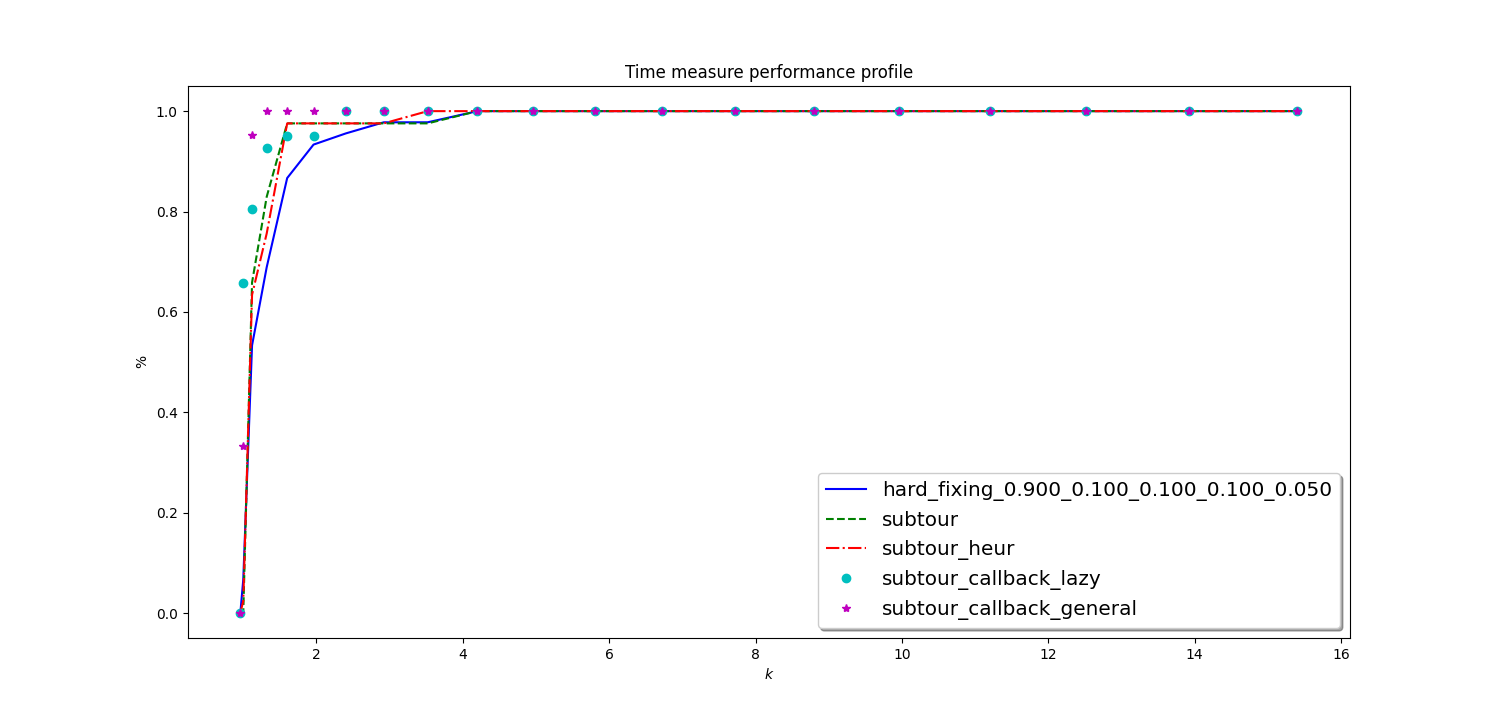
\includegraphics[width=\columnwidth]{../res/Lsubtours_hardfixing_lightaverage_time.png}
	\caption{Performance profile to compare subtours methods with \texttt{hard\_fixing}. The name of \texttt{hard\_fix} model contain in order: $ max\_f_r, incr_fr, decr\_f_r, good\_gap, optimal\_gap $. The test set is the composition of data\_light and data\_average.}
	\label{fig:Lsubtours_hardfixing_lightaverage_time}
\end{figure}


\section{Local-Branching}

\section{Tabu-Search}
Tabu Search (TS) has been developed by Fred Glover \cite{Glover1998}. TS is a heuristic that combines a local search process with a number of anti-cycling rules which prevent the search from getting trapped in a local minimum. Tabu Search is very similar to a local search algorithm that proceeds iteratively from one solution to another through the Best-2-opt \ref{sec:best_2_opt} method. It also uses a special memory structure, called a tabu list, that determines which subsequent solution will be chosen and therefore to organize the way space is explored. The algorithm starts with a random solution. By applying the Best-2-opt, as long as a new improvement solution is found, it updates the current solution to it. When it comes to a local minimum (i.e. there are no improvement solutions around two optimality) the use of the tabu list comes into play.\\
Pejorative moves are now allowed and the algorithm chooses the lowest cost one and adds this move to the tabu list, updates the current solution and starts again with the Best-2-opt.
During the next iteration, while searching for the new solution, check that the move to obtain it does not belong to the list. If it does not appear, then the move is lawful and continues with the next steps of the algorithm. Conversely, if the move is tabu (i.e. not allowed, prohibited), the solution is discarded and another is chosen, until a lawful move is found. The algorithm will continue to choose licit pejorative moves until an improvement one, that does not belong to the list, is found. In this case the algorithm starts again.\\
As will be discussed later, the tabu list has a maximum size of elements. Consequently, when a new element has to be inserted and the list is full, the "oldest" element (i.e. the one that has been inserted longer) of the list will be replaced with it.\\
This strategy allows research to move along the "hills" that the costs of the various solutions form in the solution space. It is an excellent method to escape from the local minimum by maintaining a search based on the Best-2-opt (Figure \ref{fig:tabu_search_perform_time}).\\
Looking at the implementation details there are many aspects that must be carefully evaluated:

\begin{itemize}
\item Type of structure for tabu list
\item Size of tabu list
\item Termination criterion
\end{itemize}

First of all, the type of structure used for the tabu list. We have decided to propose two different solutions, as each of them has its potential and its defects. The first, more classic, involves the use of a fixed-size array to store prohibited moves (so for each Best-2-opt move, the two relative edges are inserted into the array). The second, however, uses a linked list in which each element is formed by a variable for the edge and a pointer \textit{next} to the next element.
One of the main differences is the allocation of memory, as the linked list dynamically manages its size and therefore aims to optimize space but, on the other hand, the removal of the oldest inserted element requires complete scrolling of the list. Instead the array optimizes the operations on the elements contained but on the other hand it cannot have a dynamic dimension except through the creation and the copy in a new array (probably with an excellent knowledge of low-level memory and an ad hoc solution is possible to manage dynamic dimension of an array). For the management of the elements in the array it was decided to add one more element than the value of the chosen dimension, assigning it a static value of -1 that will never be changed. In this way, replacing an element when the list is full is very simple as it is sufficient to assign the new edge instead of -1 and replace the next element with -1. This causes the array to be cyclical and, through a single index variable, does not require any research for this type of operation.\\
Another aspect to consider is the size of the tabu list. An "infinite" dimension would risk bringing the algorithm to a standstill in which it can no longer make any move since all those around two optimality have been prohibited. Conversely, too small a size could cause a return to the local minimum from which one was running away. A lot of studies and research have been done for this specific aspect \cite{Nababan_2019, Tsubakitani1998} and a better overall result than others has not been found, changing the typology of the problem also varies the best size of the list. An average list size with respect to the problem proved to be the best choice as a balance between computational time and the optimal markspace value. Thus a size equal to half the number of problem nodes was set.\\
Finally, the termination criterion can be based on a maximum number of iterations of the algorithm or on a fixed number of iterations in which the solution no longer improves or, as in our case, on a timelimit.

\begin{figure}[h]
	\centering
	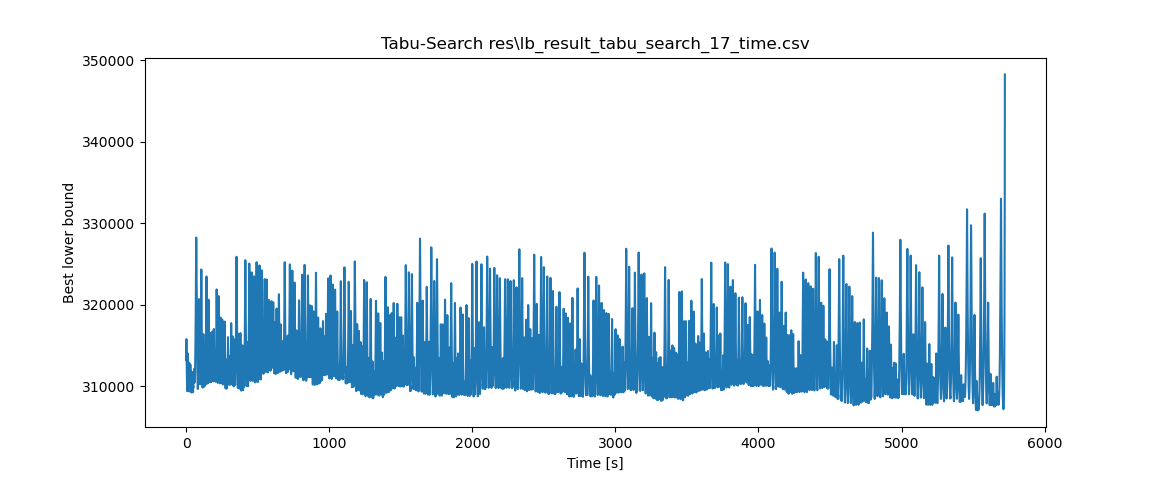
\includegraphics[width=1.0\columnwidth]{../res/gr666_17.png}
	\caption{Performance profile considering the execution time}
	\label{fig:tabu_search_perform_time}
\end{figure}

\section{Simulated-Annealing}
The goal is to find a point in the space at which a real valued energy function (or cost function) is minimized. Simulated annealing is a minimization technique which has given good results in avoiding local minima. This research is based on a Random-2-Opt (similar to \ref{sec:best_2_opt} but choose a random one instead of looking for the best one). Moreover, it follows the idea of taking a random walk through the space at successively lower temperatures, where the probability of taking a step is given by a Boltzmann distribution,
\begin{equation}
	P(\Delta E)=e^{-\frac{ E_{i+1} - E_{i}}{k \times T}}
\end{equation}
if  E\textsubscript{i+1} > E\textsubscript{i}, and p($\Delta$E) = 1 when  E\textsubscript{i+1} $\leq$ E\textsubscript{i}, with $\Delta$E =  E\textsubscript{i+1} - E\textsubscript{i} and $k$ is the Boltzmann constant. \\
A step will occur if the new energy is lower. If the new energy is higher, the transition can still occur, and its likelihood is proportional to the temperature $T$ and inversely proportional to the energy difference $\Delta$E.
The temperature $T$ is initially set to a high value (\textit{$INT\_MAX$} of \textit{<limits.h>} C class), and a random walk is carried out at that temperature. Then, the temperature is lowered very slightly according to a cooling schedule.
The cooling schedule chosen is based on the timelimit given to the algorithm, at each interaction the temperature is scaled as a percentage based on the percentage of time spent on the timelimit to perform that iteration. This avoids estimating a fixed value with which to decrease the temperature at each iteration, as the time required for an iteration can vary greatly based on the probability value found (when successful, the computational time increases drastically compared to when probability fails).\\
Furthermore, if the temperature decreases sufficiently slowly, the probability of finding the global minimum tends to 1, thanks to all simulated annealing proofs of convergence in the literature which is based on homogeneous Markov chain theory and the condition of reversibility \cite{Henderson}. Since only improvement steps are accepted at zero temperature, various Random-2-opt are performed before concluding the algorithm in order to optimize the achieved solution as much as possible.\\
The slight probability of taking a step that gives higher energy is what allows simulated annealing to frequently get out of local minima.

\begin{figure}[h]
	\centering
	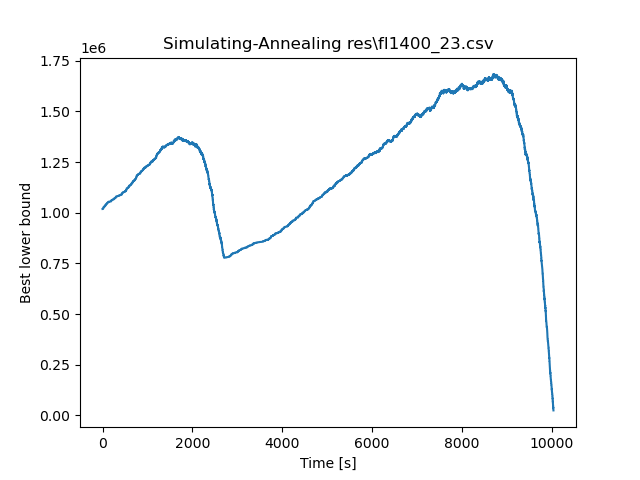
\includegraphics[width=.6\columnwidth]{../res/fl1400_23.png}
	\caption{Performance profile considering the execution time of 1400 nodes file with timelimit of 10000}
	\label{fig:simultaing_annealing_perform_time}
\end{figure}

\section{Variable Neighborhood Search (VNS)}
This metaheuristic moves from a solution to another iterating two phases:
\begin{enumerate}
	\item optimization
	\item perturbation
\end{enumerate}
The first is done iterating a refining heuristic until a local minimum is found, in this specific case it has been used the \texttt{best\_2\_opt()} algorithm, which is explained in cap \ref{sec:best_2_opt}. After the optimization, a perturbation is applied to leave the local minima, here \texttt{random\_n\_opt()} with $ n=5 $. This algorithm generate a new solution that differ n edges from the first (check at the end of the section for details).
The two phases are iterated until the max number of iterations or time limit occur.\\
Note that the implemented VNS is not optimized to work with multiple thread.\\
In fig \ref{fig:VNS_d2103} is shown the cost of the solution in each \texttt{best\_two\_opt()} step of the VNS. It is interesting to note that most of the time is required for the first descent and after that the first local minimum is found, the best lower bound does not decrease so much.
The calculated tour is plotted in fig \ref{fig:d2103_16}.\\
The performance profiles in fig \ref{fig:Lsubtour_hardfixing_vns_time} and \ref{fig:Lsubtour_hardfixing_vns_lb} show that VNS is faster than the exact algorithm and the returned solution is near the optimum.

\textbf{\texttt{Random\_n\_opt()}.} The n\_opt set of an tour T is the set of tour that have exactly n different edges w.r.t. T. \texttt{Random\_n\_opt()} return a random tour in this set.
\begin{figure}[!h]
	\begin{subfigure}{.5\columnwidth}
		\centering
		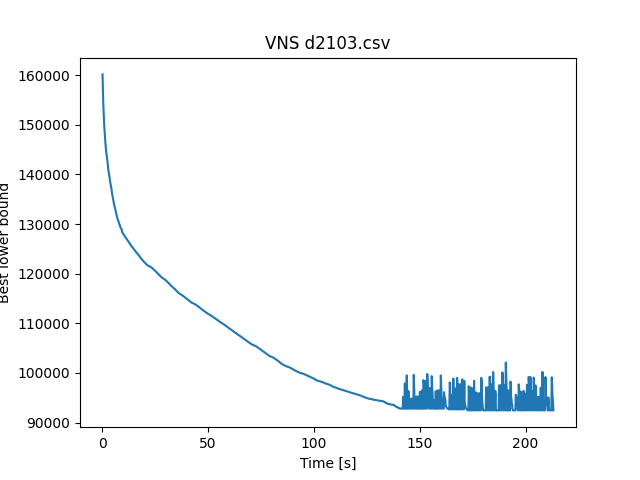
\includegraphics[width=\columnwidth]{../res/d2103.png}
		\caption{The profile of the cost of the solution (vs time domain) returned by \texttt{best\_two\_opt()} in each step of the VNS.}
		\label{fig:VNS_d2103}
	\end{subfigure}
	\begin{subfigure}{.5\columnwidth}
		\centering
		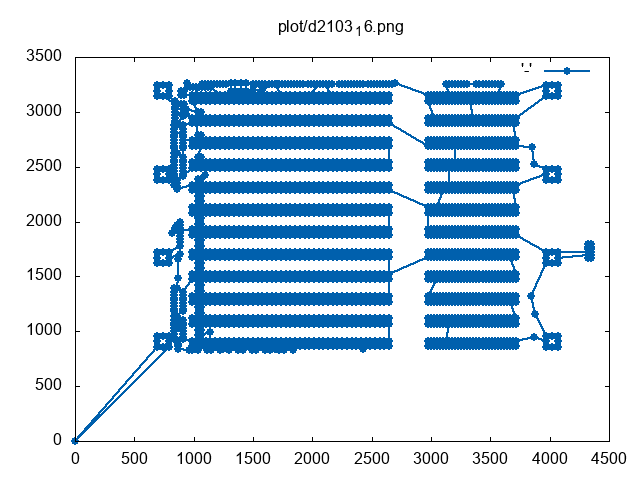
\includegraphics[width=\columnwidth]{../res/d2103_16.png}
		\caption{The graph of the solution returned by VNS.}
		\label{fig:d2103_16}
	\end{subfigure}
	\begin{subfigure}{.5\columnwidth}
		\centering
		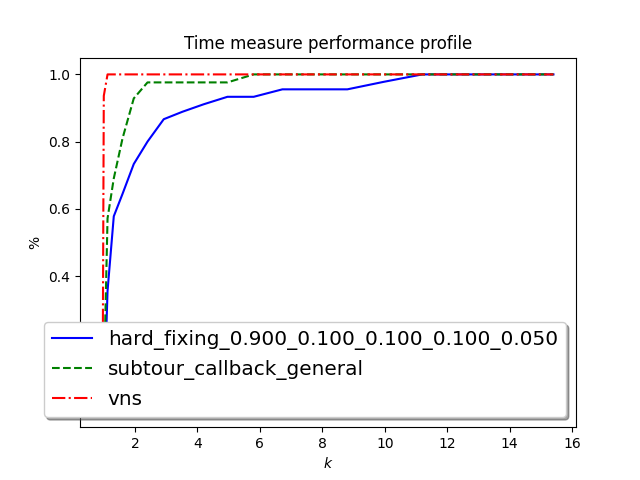
\includegraphics[width=\columnwidth]{../res/Lsubtour_hardfixing_vns_time.png}
		\caption{Performance profile considering the execution time}
		\label{fig:Lsubtour_hardfixing_vns_time}
	\end{subfigure}
\hfill
	\begin{subfigure}{.5\columnwidth}
		\centering
		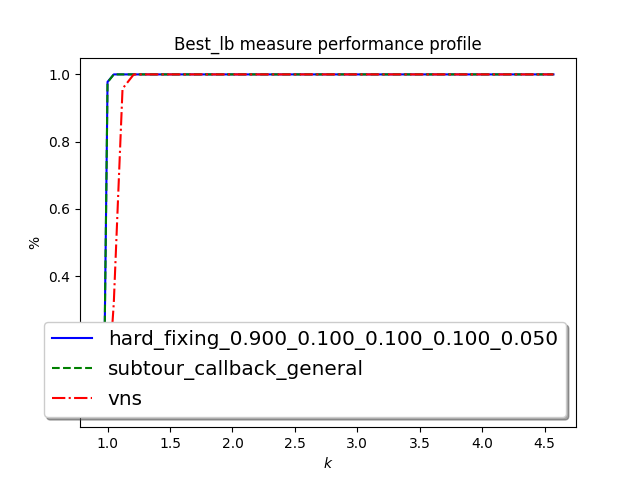
\includegraphics[width=\columnwidth]{../res/Lsubtour_hardfixing_vns_lb.png}
		\caption{Performance profile considering the lower bound.}
		\label{fig:Lsubtour_hardfixing_vns_lb}
	\end{subfigure}
\end{figure}

\section{Genetic Algorithm}
The genetic algorithm (GA) is the last meta-heuristic technique proposed. Its behaviour derives from an evolutionary biology metaphor. A population of individuals (solutions) is randomly created. The individual solutions represent one tour each. These solution are then exposed to simulated evolution.
For a complete explanation of the simple genetic algorithm, see \cite{phdthesis}.\\
A particular genetic algorithm has been implemented in this paper: it is based almost exclusively on the "Powerful Genetic Algorithm Using Edge Assembly Crossover" created by Yuichi Nagata and Shigenobu Kobayashi \cite{Nagata2013, Honda2013}, except for a subsection that has been completely designed by us.\\ A description of the algorithm will be presented and some paragraphs, which are contained in their paper \cite{Nagata2013}, will be reported here thanks to their clear description. In addition, the differences from his algorithm and our implementation choices will be explained.\\
The search process of the GA consists of two stages: \\
\begin{itemize}
\item GA-EAX/Stage I: a localized version of Edge Assembly Crossover (EAX) as the crossover operator from the start of the search until no improvement in the best solution is found over a period of generations or because of timelimit.
\item  GA-EAX/Stage II: after that, switch to a global version of EAX and use it until the end of the search. Stage II is also terminated by the same condition of previous one.
\end{itemize}
For this project only Stage I was developed but the global version does not add any difficulties in the code.

Algorithm \ref{alg:gagen} describes in a compact way the various steps of the entire search.\\

\begin{algorithm}
\caption{GA General}\label{alg:gagen}
\begin{algorithmic}[1]
\Procedure{Procedure GA()}{}
\State $\textit{\{x\textsubscript{$1$},...,x\textsubscript{N\textsubscript{pop}}\}} := \textit{INIT\_POPULATION()}$
\While{\textit{termination condition is satisfied}}
	\State $\textit{r($\cdot$)} := \textit{SHUFFLE\_INDIVIDUALS() $\equiv$ a random permutation of $1$,...,N\textsubscript{pop} } $
	\For{\texttt{$i := 1$ to N\textsubscript{pop}}}
		\State $p_A := \textit{x\textsubscript{r($i$)}} , \textit{p\textsubscript{B}} := \textit{x\textsubscript{r($i+1$)}} $
		\State $\textit{\{y\textsubscript{$1$},...,y\textsubscript{N\textsubscript{kids}}\}} := \textit{EAX\_SINGLE(p\textsubscript{A}, p\textsubscript{B})}$
		\State $\textit{x\textsubscript{r($i$)}} := \textit{SURVIVAL\_SELECTION(y\textsubscript{$1$},...,y\textsubscript{N\textsubscript{kids}}, p\textsubscript{A})} $
	\EndFor
	\State $\textit{best\_individual} := \textit{best individual of actual population}$
\EndWhile
\State \textbf{return} $best\_individual$
\EndProcedure
\end{algorithmic}
\end{algorithm}

\subsection{EAX\_SINGLE}
The recombination operator EAX uses the edges from the two parents to construct disjoint subtours.
Then, using a more general version of the Patching Algorithm \ref{section:patching}, the subtours are connected in a greedy fashion to produce the offspring tour. Thus, the EAX operator considers local information which is exploited in determining which edges to use to connect subtours.\\
Another important trait of the EAX operator is that it will introduce new edges into the offspring when connecting subtours. Edges not in the parents, or perhaps not even in the population, are introduced into offspring. 
The argument as to why good new edges must be introduced during recombination is simple. As point out in \cite{Mathias92geneticoperators}, the complete graph of all possible edges for a symmetric TSP has $(N^2-N)/2$ edges, where $N$ is the number of nodes. Each tour samples $N$ of these edges, so a population must be of size at least $(N-1)/2$ in order to sample each edge exactly once. Assume population size is proportional to the number of the nodes. Then each edge occurs twice in expectation in an initial random population. Selection can therefore quickly eliminate edges from the population. Good edges can also be lost if they occur in poor tours. Thus it is important for operators to intelligently introduce new good edges. This feature is part of the construction of EAX and therefore, may contribute to its effectiveness.\\

\begin{figure}[h]
	\centering
	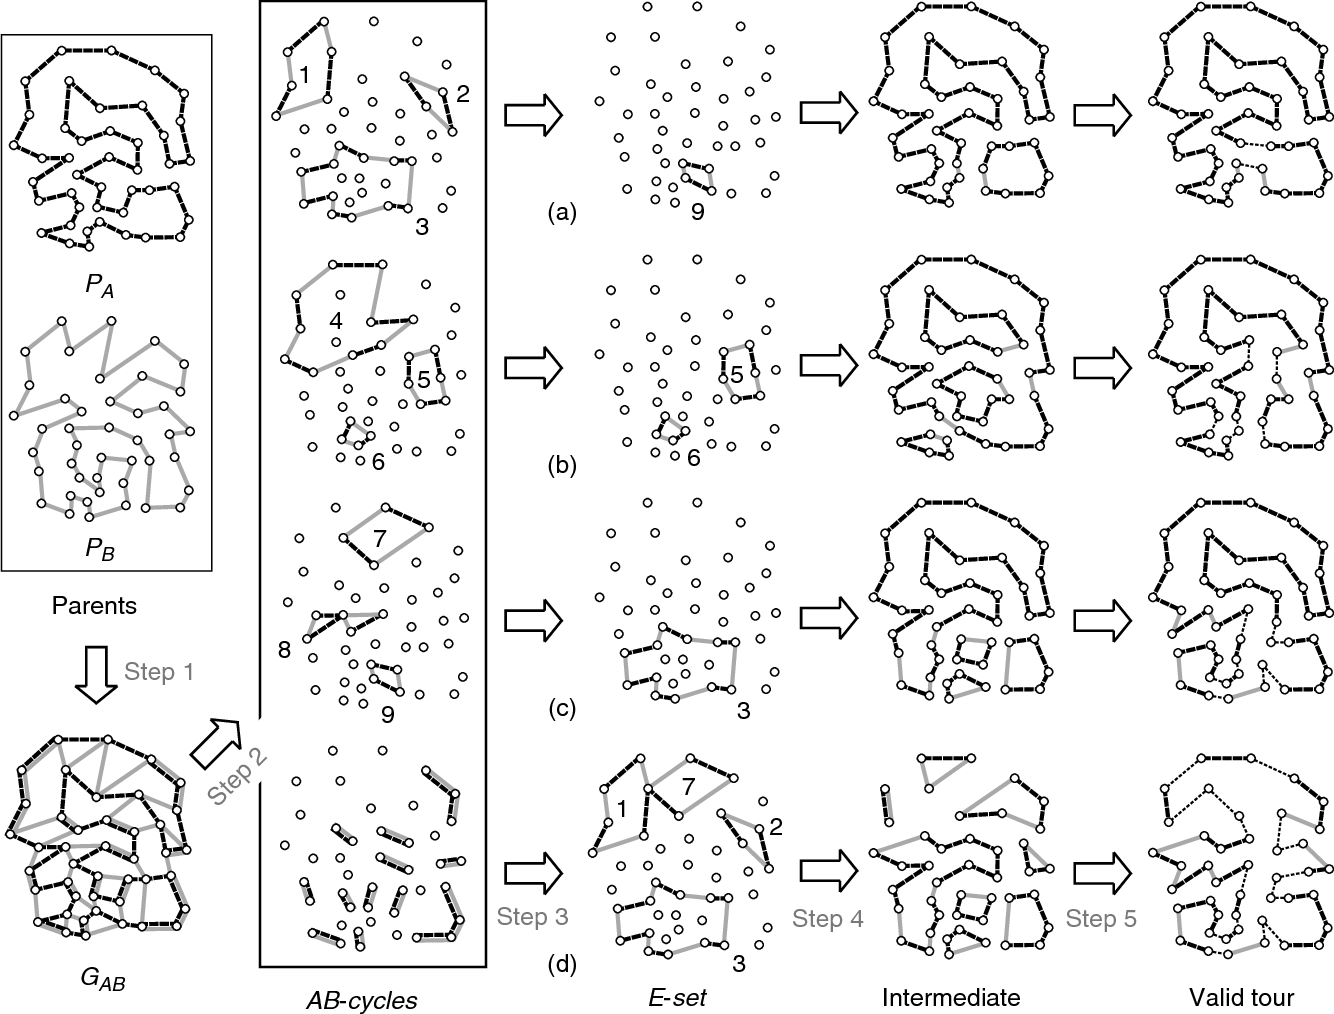
\includegraphics[width=1.0\columnwidth]{img/GA_steps}
	\caption{Example of the EAX\_SINGLE method steps (image taken from \cite{Nagata2013}).}
	\label{fig:GA_steps}
\end{figure}

Focusing on details of the EAX procedure:\\
Once two parents have been selected for crossover, the EAX operator merges these two individuals into a single graph denoted by R (Step 1 of Image \ref{fig:GA_steps}, graph R is named G\textsubscript{AB}). The two parents are denoted by A and B, respectively. Each edge in R is annotated with the parent to which it belongs. R may contain two instances of the same edge, if both parents contain the edge (that is why a more general version of Patching Algorithm is used).\\
R is next divided into a set of disjoint subtours. Let v\textsubscript{i} represent a vertex from R and let (v\textsubscript{i},  v\textsubscript{j}), i $\neq$ j, represent an edge. Suppose (v\textsubscript{i},  v\textsubscript{j}) represents an edge randomly chosen from parent A.\\
Choose one vertex (either v\textsubscript{i} or v\textsubscript{j}) as the origin. If v\textsubscript{i} is the origin, then choose an edge which leads from the second vertex, v\textsubscript{j} , to any other vertex in R. However, this edge must come from parent B. If more than one such edge exists, a random selection is made. The algorithm continues to traverse R, at each step alternately picking edges from parent A and parent B.\\
After each edge is traversed, the algorithm checks to see if adding this new edge to the set of previously selected edges will result in an AB-cycle. An AB-cycle is a even-length sub-cycle of R with edges that alternately come from A and B. An AB-cycle may repeat nodes, but not edges. While there can be two edges between a pair of nodes, they are uniquely identified as an A or B edge, and thus distinct.\\
Once an AB-cycle has been found it is stored and the edges making up that cycle are removed from R. The algorithm repeats this procedure until R contains no more edges, having been completely decomposed into a set of AB-cycles (Step 2 of Image \ref{fig:GA_steps}). \\
The first several edges used in the construction of the AB-cycle may not appear in the final AB-cycle. This occurs when the final edge connects back onto the subgraph at some node x other than the origin node, and the induced subcycle is an AB-cycle. In this case the remaining edges are however removed from R graph but is kept aside in the path being traced, to eventually be used later in forming another cycle. Nagata and Kobayashi choose an edge incident with x from R to begin construction of the next AB-cycle instead in our algorithm we preferred to take an edge incident to any node remaining in the traced path (other technique prefers to select the starting location of a new AB-cycle at random from R).
For the symmetric TSP problem, R is undirected and therefore, the set of AB-cycles is not uniquely determined by the algorithm. Furthermore, a number of "ineffective" AB-cycles may be formed by the algorithm. All AB-cycles that have less than 4 different nodes inside them belong to this group. Any ineffective AB-cycles are found and removed from R and also removed from consideration by the remaining phases of the algorithm.
\\
After construction of the set of AB-cycles, a subset of AB-cycles is chosen to be used in the generation of an intermediate child. This subset is called an E-set (Step 3 of Image \ref{fig:GA_steps}). For selecting AB-cycles for inclusion into the E-set, we choose an our method different from those defined by Nagata and Kobayashi. Given the small size of the problems we tested compared to those of the TSP Art of Nagata, the number of subtours in the E-set is not very large and therefore, instead of sampling by random selection some of them, we scroll through them all and create one intermediate child for each.
\\
Construction of an intermediate child, C, begins with a copy of parent A. Then each edge of each subtour in the E-set is examined, with the following actions taken on C. If the edge from the E-set is a member of parent A, the edge is deleted from C. If the edge is a member of parent B, the edge is added to C. The result is a set of disjoint subtours which comprise the intermediate child (Step 4 of Image \ref{fig:GA_steps}). \\
The last stage of the EAX operator involves transformation of the intermediate child into a single legal tour using a general Patching Algorithm (Step 5 of Image \ref{fig:GA_steps}). The difference between this general algorithm and the one presented in \ref{section:patching} is in the possibility of having double edges, after performing Step 4. This implies that one of the subtours can only be made up of two nodes and two same edges, one of parent A and one of B. Similar situation with three nodes and six edges (three doubles). In previous problems this situation never happened and therefore we generalized the Patching algorithm to include this variant.\\ 
The pseudocode of the EAX\_SINGLE method is identical to that explained in Algorithm 1 of Paper \cite{Honda2013}.

\subsection{Evaluate AB-Cycles}
This method was completely designed by us from scratch. It refers to how to find a cycle that respects the conditions of the EAX\_SINGLE procedure inside the nodes and edges traced so far by the current AB-Cycle. An explanation of this procedure is not given in the papers \cite{Nagata2013, Honda2013} and it is not even that simple. We initially thought of using a greedy graph search algorithm, such as Depth First Traversal (DFT) or Breadth First Search (BFS), but these algorithms do not include the presence of double edges between two nodes and are based on visiting the nodes and not edges and also once found any cycle they stop and do not provide the possibility to continue the search if the cycle does not meet certain conditions. So we have developed an ad hoc algorithm for this type of search that transforms the graph into a tree considering double edges and the possibility to continue the search if a cycle is found that does not respect the conditions required by the EAX\_SINGLE. This algorithm has a recursive structure and uses linked lists that allow a dynamic allocation to save all the necessary information, it was also built trying to free up memory as much as possible in order to avoid overflow as the generations increase. Furthermore, the possibility of finding all the cycles within the graph and not only one is managed, but, as required by the EAX, when an acceptable solution is found, the search ends.

\subsection{SURVIVAL\_SELECTION}
For the survival selection method, some parameters are defined: 

\begin{itemize}
\item N\textsubscript{pop}
\item N\textsubscript{kids}
\item Edge Frequency Table F($e$)
\end{itemize}
N\textsubscript{pop} and N\textsubscript{kids} be the population size and the number of offspring solutions generated from a single pair of parents, p\textsubscript{A} and p\textsubscript{B}, respectively, with the chosen values of 300 and 30, as in the default configuration of GA-EAX/Stage I \cite{Nagata2013}. N\textsubscript{kids} represents an upper bound to the number of offspring solutions but fewer of them could be generated. \\
The edge frequency table F($e$) is a table that records the frequencies of each edge $e \in E$ included in the population, where $E$ is the edge set of the complete graph of a given TSP instance. The values of F($e$) are initialized and are used in the evaluation function for selecting offspring solutions. This evaluation function is based on the edge entropy measure computed from F($e$) and is used for maintaining the population diversity in a positive manner. \\
To keep the table updated: let $y\ssymbol{1}$ be the selected individual among the generated offsprings, which replaces the population member chosen as parent p\textsubscript{A}. The values of F($e$) are updated as follows: 

\begin{equation}\begin{array}{ll}
F(e) \leftarrow F(e)-1 & \forall e \in E\textsubscript{remove} \\
F(e) \leftarrow F(e)+1 & \forall e \in E\textsubscript{add}
\end{array}\end{equation}

where E\textsubscript{remove} is a set of the edges that are included in p\textsubscript{A} but not included in $y\ssymbol{1}$, E\textsubscript{add} is a set of the edges that are included in $y\ssymbol{1}$ but not included in p\textsubscript{A}. \\

The offspring $y\ssymbol{1}$ is selected, taking account of the balance between the amount of the improvement and loss of the population diversity. Let L be the average tour length of the population and H the edge entropy of the population defined as follows:

\begin{equation}
H=-\sum_{e \in E} F(e) / N_{\mathrm{pop}}\left(\log \left(F(e) / N_{\mathrm{pop}}\right)\right)
\end{equation}

$\Delta$L(y) and $\Delta$H(y) denote the differences in L and H, respectively, when x\textsubscript{i}(p\textsubscript{A}) is replaced with $y\ssymbol{1}$. The offspring $y\ssymbol{1}$ is selected so that the following evaluation function is maximized.

\begin{equation}\text { Eval\textsubscript{Ent}}(y):=\left\{\begin{array}{ll}
\frac{\Delta L(y)}{\Delta H(y)} & (\Delta L<0, \Delta H<0) \\
-\frac{\Delta L(y)}{\epsilon} & (\Delta L<0, \Delta H \geq 0) \\
-\Delta L(y), & (\Delta L \geq 0)
\end{array}\right.\end{equation}

where $y$ is an offspring solution and $\epsilon$ is a sufficiently small positive number (our chosen value $0.1$).\\

\subsection{Test}

